\RequirePackage[l2tabu,orthodox]{nag}

% TODO: decide if one-sided/two-sided
%\documentclass[headsepline,footsepline,footinclude=false,fontsize=11pt,paper=a4,listof=totoc,bibliography=totoc,BCOR=12mm,DIV=12]{scrbook} % two-sided
\documentclass[headsepline,footsepline,footinclude=false,oneside,fontsize=11pt,paper=a4,listof=totoc,bibliography=totoc]{scrbook} % one-sided

\PassOptionsToPackage{table,svgnames,dvipsnames}{xcolor}

\usepackage[utf8]{inputenc}
\usepackage[T1]{fontenc}
\usepackage[sc]{mathpazo}
\usepackage[american]{babel}
\usepackage[autostyle]{csquotes}
\usepackage[%
  backend=biber,
  url=false,
  style=numeric,
  maxnames=4,
  minnames=3,
  maxbibnames=99,
  firstinits,
  uniquename=init]{biblatex} % TODO: adapt bibliography style
\usepackage{graphicx}
\usepackage{scrhack} % necessary for listings package
\usepackage{listings}
\usepackage{lstautogobble}
\usepackage{tikz}
\usepackage{pgfplots}
\usepackage{pgfplotstable}
\usepackage{booktabs}
\usepackage[final]{microtype}
\usepackage{caption}
\usepackage[hidelinks]{hyperref} % hidelinks removes colored boxes around references and links
\usepackage[toc,nonumberlist,acronym]{glossaries} % TODO: remove if glossary not needed
\usepackage{marvosym}
\usepackage{subfigure}
%\usepackage{natbib}
%\bibliographystyle{plain}
\bibliography{bibliography/literature}

\setkomafont{disposition}{\normalfont\bfseries} % use serif font for headings
\linespread{1.05} % adjust line spread for mathpazo font

% Settings for glossaries TODO: remove the following block if glossary not needed
\renewcommand{\glsnamefont}[1]{\normalfont\bfseries #1} % use serif font for glossary entry titles
\makeglossaries{}

% Settings for pgfplots
\pgfplotsset{compat=1.9} % TODO: adjust to your installed version
\pgfplotsset{
  % For available color names, see http://www.latextemplates.com/svgnames-colors
  cycle list={CornflowerBlue\\Dandelion\\ForestGreen\\BrickRed\\},
}

% Settings for lstlistings
\lstset{%
  basicstyle=\ttfamily,
  columns=fullflexible,
  autogobble,
  keywordstyle=\bfseries\color{MediumBlue},
  stringstyle=\color{DarkGreen}
}

% Basic information for cover & title page
\newcommand*{\getUniversity}{Technische Universität München}
\newcommand*{\getFaculty}{Department of Informatics}
\newcommand*{\getTitle}{Deep Learning for Sentiment Analysis}
\newcommand*{\getTitleGer}{Deep Learning Methoden für Sentiment Analysis Probleme}
\newcommand*{\getAuthor}{Ankit Bahuguna}
\newcommand*{\getDoctype}{Master's Thesis in Informatics}
\newcommand*{\getSupervisor}{Prof. Georg Groh}
\newcommand*{\getAdvisor}{Prof. Georg Groh}
\newcommand*{\getSubmissionDate}{September 15, 2015}
\newcommand*{\getSubmissionLocation}{Munich, Germany}

% TODO: add custom commands etc.


% TODO: remove if glossary not needed
\newglossaryentry{computer}
{
  name=computer,
  description={is a machine that\ldots}
}

\newacronym{sgd}{SGD}{Stochastic Gradient Descent}

\newacronym{nn}{NN}{Neural Networks}

\newacronym{svm}{SVM}{Support Vector Machines}

\newacronym{sa}{SA}{Sentiment Analysis}

\newacronym{ml}{ML}{Machine Learning}

\newacronym{nlp}{NLP}{Natural Language Processing}

\newacronym{lr}{LR}{Logistic Regression}

\newacronym{dnn}{DNN}{Deep Neural Network}

\newacronym{cnn}{CNN}{Convoluted Neural Networks}

\newacronym{rntn}{RNTN}{Recursive Neural Tensor Network}

\newacronym{msda}{MSDA}{Marginalized stacked Denoising Auto Encoders}

\newacronym{lstm}{LSTM}{Long and Short Term Memory Networks}

\newacronym{gmm}{GMM}{Gaussian Mixture Models}

\newacronym{ivec}{IVEC}{I - Vectors}

\newacronym{me}{ME}{Maximum Entropy}

\newacronym{bow}{BOW}{Bag of Words}

\newacronym{p}{P}{Polyglot Word Representation}

\newacronym{g}{G}{Glove Word Representation}

\newacronym{w}{W}{Word2Vec Word Representation}


\begin{document}

\begin{titlepage}
  % HACK for two-sided documents: ignore binding correction for cover page.
  % Adapted from Markus Kohm's KOMA-Script titlepage=firstiscover handling.
  % See http://mirrors.ctan.org/macros/latex/contrib/koma-script/scrkernel-title.dtx,
  % \maketitle macro.
  \oddsidemargin=\evensidemargin\relax
  \textwidth=\dimexpr\paperwidth-2\evensidemargin-2in\relax
  \hsize=\textwidth\relax

  \centering

  \vspace{40mm}
  \includegraphics[width=40mm]{logos/tum}

  \vspace{5mm}
  {\huge\MakeUppercase{\getFaculty{}}}\\

  \vspace{5mm}
  {\large\MakeUppercase{\getUniversity{}}}\\

  \vspace{20mm}
  {\Large \getDoctype{}}

  \vspace{15mm}
  {\huge\bfseries \getTitle{}}

  \vspace{15mm}
  {\LARGE \getAuthor{}}

  \vspace{20mm}
  \includegraphics[width=20mm]{logos/faculty}
\end{titlepage}


\frontmatter{}

\begin{titlepage}
  \centering

  \vspace{40mm}
  \includegraphics[width=40mm]{logos/tum}

  \vspace{5mm}
  {\huge\MakeUppercase{\getFaculty{}}}\\

  \vspace{5mm}
  {\large\MakeUppercase{\getUniversity{}}}\\

  \vspace{20mm}
  {\Large \getDoctype{}}

  \vspace{15mm}
  {\huge\bfseries \getTitle{}}

  \vspace{10mm}
  {\huge\bfseries \getTitleGer{}}

  \vspace{15mm}
  \begin{tabular}{l l}
    Author: & \getAuthor{} \\
    Supervisor: & \getSupervisor{} \\
    Advisor: & \getAdvisor{} \\
    Submission Date: & \getSubmissionDate{} \\
  \end{tabular}

  \vspace{20mm}
  \includegraphics[width=20mm]{logos/faculty}
\end{titlepage}

\thispagestyle{empty}
\vspace*{0.8\textheight}
\noindent
I confirm that this \MakeLowercase{\getDoctype{}} is my own work and I have documented all sources and material used.

\vspace{15mm}
\noindent
\getSubmissionLocation{}, \hspace{5cm} \getAuthor{}
\newline
\getSubmissionDate{}
\cleardoublepage{}

\addcontentsline{toc}{chapter}{Acknowledgments}
\thispagestyle{empty}

\vspace*{2cm}

\begin{center}
{\usekomafont{section} Acknowledgments}
\end{center}

\vspace{1cm}

%TODO: Acknowledgments
I would like to wholeheartedly my supervisor \textbf{Mr. Georg Groh}, who advised my Master's Thesis at TUM and kept me encouraged during the whole time. He played a pivotal role in me continuing the study in the area of my interest and help me chase the state of the art systems with utmost frivolity. I would also thank, \textbf{Prof. Hinrich Schütze}, with whom, I started this study with an interdisciplinary project at Ludwig Maximillian's University (München) and his supervision helped me to get started with the new topic of Deep Learning and its application to Natural Language Processing. Additionally, I would thank my previous guide, \textbf{Prof. Pushpak Bhattacharrya},(Indian Institute of Technology, Bombay) who introduced the field of Natural Language Processing and helped kick-start my interest in the field and encouraged me continuously to aim higher and helped me open my mind to look at problems from various perspectives..  

In the end, I would also like to thank my family, who gave me this opportunity to study at Technical University of Munich, Germany. Without them, nothing of this would be possible. 
\cleardoublepage{}

\chapter{\abstractname}

%TODO: Abstract



\microtypesetup{protrusion=false}
\tableofcontents{}
\microtypesetup{protrusion=true}

\mainmatter{}

\chapter{Introduction}\label{chapter:introduction}


\section{World of Opinions and Sentiment}
"\textit{What other people think}", has been a very important element in the overall decision making process.~\parencite{pangleesentiment} This is more relevant in the modern era with the explosion of web and internet based services where the people have a new platform where they can voice their opinions and discuss about day to day things. With the advent of this platform, the subjective information too has grown extremely rapidly over the years.  
\newline

It is interesting to note that social opinion of users impact a large corpus of audience. A simple case example is, that if a product is negatively perceived in the social circles of the internet, it will not be taken positively by a new user who is interested in purchasing the product. Hence, this is also a tool for organizations to understand how the product is performing in the public. This, has given rise to a new area of study known as social media monitoring and analysis. 
\newline

In the modern day, organizations have made significant investments to process this vast amount of data and make sense of the important information contained in it, so that they can leverage their products and services and improve their overall user experience or increase chances of making more profit, by identifying key areas which are causing an indirect impact on the overall profit margin. In the modern world, the organizations which makes the best use of data is the clear winner and it also is an opportunity for the researchers working in the area to aggressively pursue new techniques and algorithms which beat the current state of the art systems, giving the organizations slight edge over their competitors, which can in turn bring millions of dollars in revenue.      
\section{Sentiment Analysis: An Introduction}
It's well said that the fundamental difference, between a human and a computer is that, the computer doesn't perceive or express emotions. If someday, this barrier can be overcome, then it will be very hard to distinguish a human conversation  from a machine conversation. Thus, the broad goal for the study of Sentiment Analysis, is making computers recognize and express emotions.  

First, we present some of the common terms, which are regularly used in context of Sentiment Analysis, viz., \textbf{opinion}, \textbf{sentiment} and \textbf{subjectivity} in text. These can be defined in the following manner:
\newline

\textbf{opinion} : \textit{A view or judgment formed about something, not necessarily based on fact or knowledge.}
\newline

\textbf{sentiment} : \textit{A view or opinion that is held or expressed.}
\newline

\textbf{subjectivity} : \textit{Refers to how someone's judgment is shaped by personal opinions and feelings instead of outside influences. }
\newline

The term opinion mining appears in a paper by Dave et al. \parencite{ch1:dave}. Interestingly, an ideal opinion-mining tool would "process a set of search results for a given item, generating a list of product attributes (quality, features, etc.) and aggregating opinions about each of them (poor, mixed, good).” 
\newline

The history of the phrase sentiment analysis parallels that of “opinion mining” in certain respects. The term “sentiment” used in reference to the automatic analysis of evaluative text and tracking of the predictive judgments therein appears in 2001 papers by Das and Chen ~\parencite{ch1:daschen} and Tong ~\parencite{ch1:tong}, due to these authors’ interest in analyzing market sentiment. It subsequently occurred within 2002 papers by Turney ~\parencite{ch1:turney} and Pang et al.~\parencite{ch1:pang}, which were published in the proceedings of the annual meeting of the Association for Computational Linguistics (ACL) and the annual conference on Empirical Methods in Natural Language Processing (EMNLP). These papers really increased the popularity of the term "Sentiment Analysis" in the Natural Language Processing research community. A number of papers mentioning “sentiment analysis” focus on the specific application of classifying reviews as to their polarity (either positive or negative), a fact that appears to have caused some authors to suggest that the phrase refers specifically to this narrowly defined task. However, nowadays many use the term more broadly to mean the computational treatment of opinion, sentiment, and subjectivity in text. A famous and more comprehensive account on this subject was presented by Bo Pang and Lillian Lee\parencite{pangleesentiment} \parencite{ch1:pang} which covered the various techniques and approaches that promised opinion oriented information seeking systems. This work accounted a full fledged review, which this current literature also follows in parts in the first two chapters.
\newline

If we look in a broad view, the terms sentiment analysis and opinion mining roughly imply the same field of study, which itself can be attributed as the sub field of subjectivity analysis. For the sake of simplicity, we will stick to "sentiment analysis" throughout this work. 

\section{Applications}
There are a number of application areas of this study, although, in the introduction we have mentioned reviews related to websites and products but in general there are many other possibilities. It is because of all the possible applications, there are a good number of small startups to large organizations which have dedicated teams who look into this subject matter and have it as part of their mission statement.


\subsection{A Review based Search Engine}
A classic example can be a review oriented search engine. Consider a product search engine which also utilizes the reviews on the products made. And ranks the result based on the positive polarity of the products. Thus, the products which has maximum positive  product reviews are ranked higher than the ones which receives lower reviews. This will help a client who is user of the search engine to have high confidence about the kind of products returned. Such a search engine will in a way give an assurance to the customer that the best reviewed product which are socially favorable and appreciated are shown first to the user, hence making it easy to make the final choice of eventually purchasing the product. 

\subsection{Websites hosting Reviews}
There is a growing number of opinion hosting websites, for example, epinions.com; along with the booming e-commerce industry which showcase products and offers, there are millions of reviews generated every week. Thus, they are a primary playground for sentiment analysis. These can be a good benchmark for the companies to evaluate how the product is performing in the market. By performing a comprehensive analysis of the reviews which are hosted on these websites, the companies get a fair idea about the pros and cons about their product and also about the competitor. A general sentiment about the public perception can help organizations make important decisions about how to go or not go about the future iterations of the projects. Some organizations, perform a real time analysis, so that if a feature is causing a universal cry, resources can be quickly put together into immediately fixing the issue and thus leveraging overall user experience, leading to a longer user loyalty retention.

\subsection{Sub-System Technology}
Sentiment analysis can also be used a sub-system leveraging the effectiveness of another intelligent computational system. One possibility is the augmentation to a \textit{recommendation system}. Thus, a recommendation system will utilize a sentiment analysis system, which can then not recommend products which receive a lot of negative feedback.  

\textit{Detection of overheated or agnostic  language} in emails or any other form of communication is another use of subjectivity detection and classification. 

In \textit{online systems and display advertisements}, where its required to display advertisements relevant to the content of the web-page and some may contain sensitive material, it always better is such sensitive websites can be  recognized in advance. A more sophisticated system can display an advertisement when more positive statements in content are discovered and nix the same when negative statements begin to appear. 

Also in \textit{information extraction} which is heavily based on objectivity in text, can leverage subjectivity detection and discard any subjectivity content, thus improving overall quality of information extracted.  

\textit{Question Answering systems} can also be improved, as the opinion oriented questions can be handled differently. These questions differ in the subjective sense and a pre-analysis of the same can be useful to generate better answers. Similarly, \textit{summarization} can also be made useful in the context of the multiple views points.  

In the area of citation analysis, where potentially, one can detect whether the citation done by the researcher in his scientific work is a support or a rebuttal of the cited work.

\subsection{Business and Government Intelligence}
Sentiment Analysis is used effectively as a business intelligence tools. The reviews about the product can be indicative directly what is right or wrong about the product or it may be useful to mine the reviews from all the general domains like opinion websites,blogs, public forms and product pages and summarize each f the review entities corresponding to each product thereby giving a consensus of all the key points relevant in the eyes of the users with respect to the product. The data can also determine what are the current trends in the given business category and can be used to leverage the key insights which in-turn can benefit sales.  

With a view point of government  Intelligence, such a tool can be used to monitor hostile behavior in a communication. This form of government intelligence can help in also beefing up security if a known threat is determined in advance.

\subsection{Inter-Domain Applications}
Sentiment Analysis has not only been cherished by computer and data scientists but also in the political circles of the government. It has actually turned out to be a golden tool in political elections. Knowing what the people think about the candidates in a general election can allow a party to choose the right candidate and also work on its shortcomings in due time, to win the ever significant final elections. 

Moreover, there are now e-portals which are facilitating \textit{eRuleMaking}, where a new policy is first open to the public and then based on the various opinions of the general public, the decision to move forward and cement the proposed rules into a law or updating its various sections is taken into consideration. This has proved to be an effective tools to iron out any problems which may exist in a proposed law even before its presented to the democratic authority. Thus, saving both time and resources.

\section{General Challenges}

Often a simple question comes to mind, when discussing Sentiment Analysis: \textit{How is it different from classic text mining and fact based analysis?}

Traditionally, text categorization involves categorizing text into categories. These categories can be topics which are either predefined or looked up as more data is processed. These categories can also be user or application specific. And, for a given task, we might be dealing with wither a two class or binary classification or a multi-class classification (say, among thousands of classes).   In contrast, with sentiment analysis, we are usually focused with 3 classes: positive, negative or neutral (coarse grained) or, 5 classes: positive, slightly positive, negative, slightly negative and neutral (fine grained).  Thus, the number of classification classes are fairly limited and it generalizes well to many information domains and users. moreover the topics or categories can sometimes be highly non-correlated whereas the sentiments classes are often opposite in nature (in case of binary: positive- negative classification.)

Also, there is fundamentally a difference when it comes to answering opinion oriented questions vs fact based questions. The traditional information extraction methods which work well for a number of facts based templates. An opinion oriented information extraction method too will be a generalized version of the traditional system, as they are focused on similar fields of an opinion expression (holder, type and strength) irrespective of the topic. Although, it may seem the propositions presented above may make the task of sentiment analysis relatively easy, but its far from the actual truth. We will learn next about the difficulties in developing sentiment analysis systems, as compared to traditional fact based text analysis systems.

\subsection{Difficulty in Sentiment Classification?}
First, we start with a simple scenario and a connected question: Given, we have an opinionated sentence in some given language, our task is to classify it into one of positive, negative or neutral classes. How hard is this overall task?
Let's start with some examples:

1. It was a great restaurant.

2. It should have been a great restaurant.

3. The restaurant was great in that it will make all future meals seem more delicious.

4. Despite a pleasant experience I can’t support the many reviews that it was a great restaurant.

First sentence is a positive sentence, implied by "great restaurant", The rest of the sentences are all negative. But there exists a varying degree of negativeness among them. The second sentence with the phrase "should have been" implies the desired result. Which suggests that the restaurant was expected to be better than it actually was. The third sentence is a classic case of saracasm. This is hardest to spot even for humans; On the first glance we might be mistaken to consider this as positive. Sentence 4, started with a positive vibe "pleasant experience", but the reviewer then retracts his support to all the positive reviews made about the restaurants by others, thus making his overall review negative. 

These four sentences just provide a glimpse to how hard is to analyze sentiment. Moreover, apart from detecting polarity in subjective sentences, there is something, which is known as beyond polarity analysis, where the task is to detect more expressive features like anger, happiness, sadness and relaxation in text, these too are very hard to predict and are highly context driven. The context may be based on the expression in the sentence or say, in a conversation among two individuals, their relationships between them. For example, the sentence "Your're a Liar!", may mean either positive or negative given the two individuals and their relationships. Like, a candid conversation between a couple, one may take this in positive sense (not always!), but among politicians it certainly means seems negative. 

Then there is also a problem of \textbf{entity level sentiment} and \textbf{domain specificity}. The sentiment of a reviewer of a product may be dependent on individual entities composing a product. Say, for example: A user is writing a review about a \textbf{digital camera}: 

\textit{``I consider this is as a decent looking camera. The lens is of high quality and performs well in low light condition. Although, the flash is timely, it just seems to fade away the colors. There is also the issue with the battery which only takes about 100-150 photos on full charge, making periodic recharging necessary. Last, the price is the reason, I won't recommend this camera to anyone, because there are other better cameras for the same specs and lower price which are better buy in the category. "}

In the above review, the user is highly positive about the looks and lens of the camera. Thus, the review begins on a positive note and then the user comments about the flash, battery and the price, eventually making the review a negative one. This example is essentially useful in understanding the complexity involved in extracting the overall sentiment of a long review. Such long reviews are common in the real world and thus, this task is harder than it seems. Often, in such cases, it's best to understand what entity or sentence contributes the most to overall sentiment. Although, this is easier said than done! 

One may, also find that the specific qualities of the entities, which seem good for a certain product may not be good for another. This is where domain specificity is required. For example,
\begin{itemize}
\item  “\textbf{unpredictable}” may be negative in a car review, but positive in a movie review~\parencite{ch1:turney}
\item “\textbf{cheap}” may be positive in a travel/lodging review, but negative in a toys review
\end{itemize}

In this current work, we are more concerned about determining the orientation of an opinionated text. We assume that the sentences which we analyze are subjective in nature and express opinions. If, that were not the case, we wold have to first filter out opinion-centric sentences from the non - opinionated or objective sentences. This type of analysis is more specifically subjectivity analysis and goes beyond the scope of this work. In simple terms, sentiment classification is a sub-field of subjectivity analysis.

Next, we dig deeper into the problem and discuss some relevant methods which have been developed over the years to solve problems related to sentiment classification.   
\chapter{Sentiment Analysis}\label{chapter:sentiment}
Till now we have studied about Sentiment Analysis with a general perspective. This chapter starts a more computational view of solving this problem. Before we begin discussing various methods, its important to understand the scope of the problem. 
\section{Sentiment Analysis Levels}
The sentiment analysis problem is not a single view problem, rather its can be viewed as multi-level problem. They are discussed as follows:
\begin{itemize}
\item \textbf{Document Level: }Identifying if the \textit{document} (product review, blog-post, forum post etc.) expresses opinions and if they do, classifying them as positive, negative or neutral. this takes into account the overall sentiment expressed by the opinion holder for the whole document.  
\item \textbf{Sentence Level: }Identifying whether a single \textit{sentence} is positive, negative or neutral.
\item \textbf{Attribute Level: }Extracting the \textit{object attributes} (image quality, zoom size etc.) that are subject of an opinion and the opinion orientation.

It is important to note here that as the object becomes more granular, the intensity or difficulty of sentiment analysis increases.
\end{itemize}

\section{Document-Level Sentiment Analysis}
We start with the traditional methods for document analysis sentiment analysis. It's important to keep in mind few assumptions which come along the way. 
\begin{itemize}
\item The document is opinionated on a single object
\item the opinions are from a single opinion holder.
\end{itemize}
In real world data, these assumptions don't usually hold. But, for the sake of simplicity, we start with them to make the understanding of the methods easy.

Also, more importantly,  this analysis is slightly different from the topic based text classification. In topic classification, heavy emphasis is given to the extraction of the topics. Thus, the \textit{topic words} become very important.  Whereas, in sentiment classification, the opinion words are more important. For example: wonderful, fabulous and terrible. 

So to start with, a naive sentiment classifier can be based on identification and processing of these opinion words. Opinionated words are also known as sentiment words, opinion lexicon, polarity words or opinion bearing words. They are categorized into two types. First, \textbf{Base types}, for example:

Positive: wonderful, elegant, amazing

Negative: horrible disgusting poor

Second, Comparative Types, for example: better, worse etc.

\subsection{Counting Opinion Words}

We start with a simple method. We try to count the opinion words in a given document. We are given an opinion word list which have both positive and negative words. And we assign an \textbf{orientation score} (-1,1) to all words in this list. Such that, \newline

Positive opinion words (+1): great, amazing, love ...

Negative opinion words (-1): hate, horrible, etc ...

Strength of these words can also be defined [0,1] 
\newline

Thus the orientation score for the document, is the sum of the orientation scores of all opinion words found. Lets, take an example review and count the opinion words in the same and calculate overall orientation score for that review. Example:

“My Canon Powershot takes \textbf{great} pictures! ... My friend had gotten one about a year ago and she \textbf{loves} it. So, after seeing her enthusiasm about it I decided to get one and I will never go back to any other camera. I absolutely \textbf{love} this camera. I believe that every person on Earth should own one of these. ... It is \textbf{amazing}! ... There is not one thing I \textbf{hate} about this product, which is strange because I am a very picky person! ...”

Positive Sentiment Words: great (1), love (2) and amazing (1); Total: 4

Negative Sentiment Words: hate (1); Total: 1
\newline 

Overall Sentiment Orientation for Review = 4-1 = 3 or \textbf{Positive Review Overall}!

After looking at this analysis, lets ask ourselves a question. \textbf{Is simply counting the opinion words good enough?}

The answer to that is \textbf{NO}! Lets' see why. Just take into consideration the last sentence in the above review. 

There is \textbf{not} one thing I \textbf{hate} about this product. $\rightarrow$ Not Negative!
\newline

This is positive sentence overall. Since, we only captured our negative sentiment word \textbf{"hate"}, we labeled this sentence as negative, which is not true. Because of the negation indicator "not", the sentiment is reversed as in  \textbf{not ... hate} $\Rightarrow$ \textbf{like}.. Thus, an important lesson here is that we need to handle negation.  A common pattern of analysis is:
\newline

"not ... \textbf{negative}" $\rightarrow$ \textbf{positive}

"never ... \textbf{negative}" $\rightarrow$ \textbf{positive}
\newline

Thus, the overall orientation score of the review is 4 +1 = 5 and not 3 as stated previously.
\newline

\textbf{A word of caution:} Negation must be handled very carefully! As, "not" in the pattern: "not only ... but also" does not change the orientation. 

\subsection{Rule Based Method}

Another method to compute the overall sentiment of a document is through handcrafted rules which are provided by a trained linguist, based on the identification of linguistic phenomenon which determine sentiment for a given language. We first discuss some related terminology:
\begin{itemize}
\item \textbf{Pattern / Rule:} A sequence of tokens.
\item \textbf{Token:} An abstraction of a word, represented using lemma, polarity tag or a part of speech tag. There are two special tokens. TOPIC: an attribute (ex. weight, size etc.) and GAP\_DIGIT\_DIGIT: How many words can be skipping between two tokens to allow more tolerant matching. Ex GAP\_1\_2 
\item \textbf{Polarity Tag:} positive, negative, neutral, NOT (negation)
\item \textbf{POS Tag:} NN (Noun), VB (Verb), JJ (Adjective), RB (Adverb), IN (preposition) ...
\end{itemize}

Examples of some basic opinion rules, Label Sequential Pattern (LSP) Matching:
\begin{itemize}
\item Subject {like | adore | want | work} TOPIC $\rightarrow$ positive, e.g. – ``I like the old camera”
\item Subject {is | are} {great | fantastic | simple | easy} $\rightarrow$ positive, e.g. – ``This camera is fantastic”
\item TOPIC GAP\_0\_3 NOT work $\rightarrow$ negative, e.g. – ``The new search still does not work”
\item Please do NOT VB $\rightarrow$ negative,e.g. – ``Please do not roll out this new search!”
\item NOT GAP\_0\_3 {want | think | believe | need | get} $\rightarrow$ negative, e.g. – ``I do not want large size pictures in the Gallery window.”
\item {get | bring | give | put | change} GAP\_0\_3 TOPIC GAP\_0\_3 back $\rightarrow$ positive
– ``Please put the old search and browse back!”
\end{itemize} 

Although this method seems to work pretty well, but there is a fundamental limitation in putting it to use at large scale. Any rule based mining methods are computationally expensive. In this case, only a limited number of opinionated words are found and only a limited number of patterns can be created. 

Note that there are methods, which are helpful in generation and classification of these sentiment words automatically, but we do not go deeper into the same. For the more curious, some methods which are used for this purpose are discussed in the works of Turney 2002 which make use of PMI (Point-wise Mutual Information), Dictionary based methods (SentiWordnet), Corpus based Methods (which rely on syntactic of co-occurrence patterns in large text corpora) etc. 

TODO: Refer several related papers here! 

\subsection{Supervised Machine Learning Techniques}
\subsection{Domain Adaptation}

\chapter{Deep Learning}\label{chapter:deeplearning}

\section{Foundations: Neural Networks}
\section{From Neural Networks to Deep Neural Networks}
\section{Applications}
\chapter{Deep Learning and NLP: Distributed Representations and Language Modelling}\label{chapter:deepnlp}
Most, of the current Deep Learning research in NLP is focused on representation learning. By that, we mean that we represent our word, phrase or a sentence as a series of numerical values or a vector in a given vector subspace, which somehow captures the representation. This is an extensive area of research and the roots are based on the concept of Language Modeling.  
\section{Language Modelling}
A language model is a probabilistic model that assigns probabilities to any sequence of words. Such as: 
\begin{center}
\textit{p(${w}_{1}$, ... , ${w}_{T}$)}
\end{center}
Language modeling is the task of learning a language model that assigns high probabilities to well formed sentences. We take into consideration: nth order Markov assumption, where we assume that the ${i}^{th}$ word was generated based only on the n-1 previous words. It plays a crucial role in speech recognition and machine translation systems. 

\begin{figure}[ht!]
  \centering
  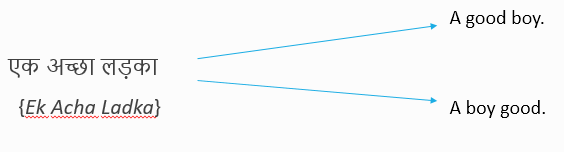
\includegraphics[height=25mm,  width=80mm]{figures/4_languagemodellingex.png}
  \caption[Language Modeling Example]{Translation of a Hindi language Sentence to English language }
  \label{languagemodellingex}
\end{figure}

Consider the example in \autoref{languagemodellingex}. We can see that the Hindi language sentence can be translated in two different ways. First, \textit{A good boy} and second,  \textit{A boy good}. What a good language model will tell us that the first one is the correct and more generally used form of the sentence. This is the power and importance of language modeling and is in the heart of all the current unsupervised natural language processing machine learning algorithmic tasks.

\subsection{Language Modelling using Ngrams}

An N-gram is defined as a sequence of n-words. For example:

\textbf{unigrams} (n=1): “is’’, ‘‘a’’, ‘‘sequence’’, etc.

\textbf{bigrams} (n=2): [‘‘is’’, ‘‘a’’ ], [‘‘a’’, ‘‘sequence’’ ], etc.

\textbf{trigrams} (n=3): [‘‘is’’, ‘‘a’’, ‘‘sequence’’], [ ‘‘a’’, ‘‘sequence’’, ‘‘of’’], etc.

The \textbf{n-gram models} estimate the conditional from n-grams counts.

\begin{center}
$P({w}_{t} | {w}_{t - (n-1)}  , ...... , {w}_{t-1}) = \frac{count({w}_{t - (n-1)}  , ...... , {w}_{t-1}, {w}_{t} )}{count({w}_{t - (n-1)}  , ...... , {w}_{t-1})}$

\end{center}
The counts are obtained from a training corpus (a data-set of word text)

We want the value of \textbf{n} to be large, for the model to be realistic. But, for large values of \textbf{n}, it is likely that a given n-gram will not have been observed in the training corpora. Smoothing helps but only partially!

\subsection{Word Representations}
In context of current problem, we use usupervised deep learning techniques, to learn a word representation C(w) which is a continuous vector and is both syntactically and semantically similar. 
More precisely, we learn a continuous representation of words and would like the distance $||C(w)-C(w’)||$ to reflect meaningful similarity between words \textbf{w} and \textbf{w’}.

Chiefly, we explore the following word representations: Word2Vec, Polyglot, GloVe and their concatenated combinations along with Bag of Words representation and compare their results for the task of sentiment analysis.
\newline

A traditional view of the word representation is the \textbf{bag of words} or \textbf{one-hot vector} representation for the word. In this model, a text (such as a sentence or a document) is represented as the bag (multi-set) of its words, disregarding grammar and even word order but keeping multiplicity. Example: Suppose we have two documents D1 and D2
\newline

\textbf{D1:} \textit{John likes to watch movies. Mary likes movies too.}
\newline

\textbf{D2:} \textit{John also likes to watch football games.}
\newline

\textbf{Vocabulary \{Word : Index\}}
\newline

{   "John": 1,    "likes": 2,     "to": 3,     "watch": 4,     "movies": 5,     "also": 6,     "football": 7,     "games": 8,     "Mary": 9,     "too": 10 }
\newline

There are 10 distinct words and using the indexes of the Vocabulary , each document is represented by a 10-entry vector:
\newline

\textbf{[1, 2, 1, 1, 2, 0, 0, 0, 1, 1]}

\textbf{[1, 1, 1, 1, 0, 1, 1, 1, 0, 0]}
\newline 

There is a concern that in this representation, the more frequent words are weighted more than less frequent words. So, to normalize the weights across documents another representation called TF-IDF (Term Frequency - Inverse Document Frequency) is introduced.The main cause of concern with BOW and TF-IDF representation is they don't make the use of contextuality of words in the corpus. Thus, there is no way of distinguishing the order of the words correctly through this vector representation. A more recent view on this is taken through neural language modeling and it brings forward a new concept known as \textbf{Word Embeddings}. On the contrary to the one-hot representation, they build on a concept of \textbf{Distributed Representations}.
\newline

Originally, word embeddings were introduced by Bengio et al., ~\parencite{bengio1} ~\parencite{bengio2} a few years before the discussed 2006 deep learning renewal, at a time when neural networks were not that popular. Although, the idea of distributed representations for symbols is much more older, as proposed by Hinton et. al.~\parencite{hinton1}  

A \textbf{word embedding} \textit{W} : words $\Rightarrow {R}^{n}$ is a paramaterized function mapping words in some language to high-dimensional vectors (150 - 600 dimensions). For example, we might find:

W(‘parrot") = (0.3, -0.5, 0.7, ...)

W(‘‘carrot") = (0.0, 0.6, -0.1, ...)
\newline

Typically, the function is a lookup table, parameterized by a matrix, $\theta$, with a row for each word: ${W}_{\theta}({w}_{n})={\theta}_{n}$. W is first initialized randomly for each word. When we train the word vector matrix, it learns to have meaningful vectors in order to perform some task.
\newline

For example, we can train a neural network to predict whether a 5-GRAM (sequence of five words) is correct or 'valid'.  We can start with 5-grams from Wikipedia corpus (Ex.. “plane is going to fly”) and then corrupt half of them by switching a word with a random word (eg. “plane is drunk to fly”), thus, almost certainly making our corrupted 5-gram absolute nonsense.The neural network we train will feed each word in the 5-gram through W to get a vector representing it as intermediate output and feed those intermediate results into another layer say 'L' which tries to predict if the 5-gram is ‘valid’ or ‘corrupt.’~\parencite{bottou} We would obtain something like:
\newline

L(W("plane"), W(‘‘is"), W(‘‘going"), W(‘‘to"), W(‘‘fly"))=1
\newline

L(W("plane"), W(‘‘is"), W(‘‘drunk"), W(‘‘to"), W(‘‘fly"))=0
\newline

In order to predict these values accurately, the network needs to learn good parameters for both W and L. This is accomplished through back-propagation, which we have already covered earlier.
\newline

An interesting side effect which is observed, with these word vectors, is when trained on a very large corpus like Google News, the vectors for days like Tuesday and Wednesday fall close to one another in high dimensional space.  It's not just limited to days, but also gender, where the same gender words fall in a certain cluster group and difference between the tow gender entities is captured across relations. For Example:
\begin{center}
\textit{v("king") - v("queen") = v("man") - v("woman")}
\end{center}
These are interesting relationships which are somehow giving the sense that they capture the semantic similarity in vector space. Thus, with such results, the entire field of Deep Learning and NLP looks really fascinating. Next, we will discuss some of the recent methods, which have contributed strongly to this discussion.

\section{Word2Vec}
Mikolov et. al. proposed two novel architectures~\autoref{w2vmodelarch} ~\parencite{mikolov1}~\parencite{mikolov2}  for computing continuous vector representations of words from very large datasets. They are:
\begin{itemize}
\item Continous Bag of Words (cbow)
\item Continous Skip Gram (skip)
\end{itemize}

\begin{figure}[ht!]
	\centering
		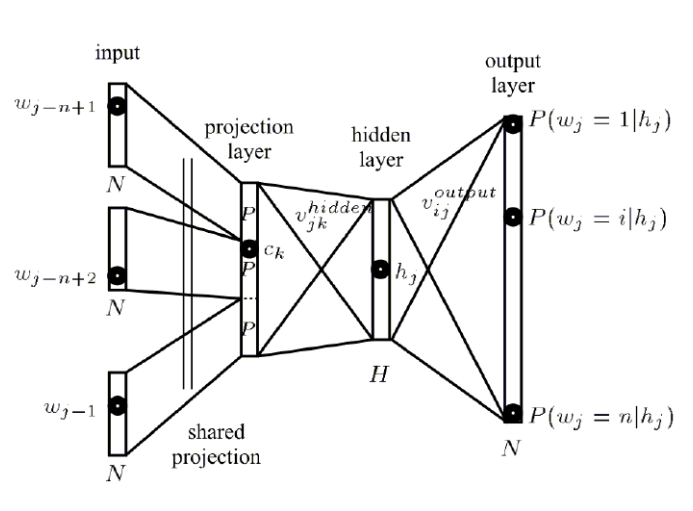
\includegraphics[height=65mm,  width=100mm]{figures/4_languagemodelnn.png}
		\caption[Word2Vec Neural Network Model]{Word2Vec Neural Network Language Model}
			\label{languagemodelnn}
\end{figure}


Word2Vec focuses on distributed representations learned by neural networks~\autoref{languagemodelnn}.  The N-previous words are encoded using 1-of-V hot-vector coding. The words are then projected by a linear operation on the projection layer. Softmax function is used at the output layer to ensure that 0 < = p < = 1. All models are trained and weights are learned using stochastic gradient descent and back propagation. For all models, the training complexity is proportional to:
\begin{center}
 O = E x T x Q,
 \end{center} 
Where, E: \# of Training epochs; T = \# Words in Training Set; Q = Defined further for each model architecture. 

\begin{figure}[ht!]
	\centering
		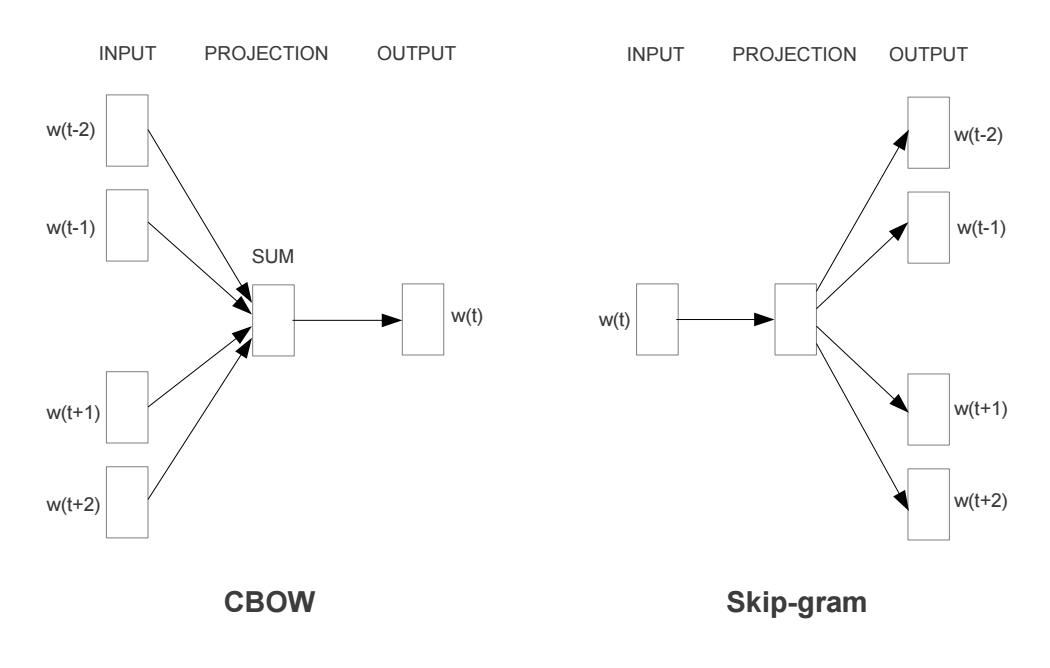
\includegraphics[height=65mm,  width=100mm]{figures/4_w2v.png}
		\caption[Word2Vec Model Architectures]{Word2Vec Model Architectures: CBOW and Skip-Gram}
			\label{w2vmodelarch}
\end{figure}

\textbf{CBOW}: Predicts the current word based on the context.
\begin{itemize}
\item Similar to feed-forward neural network language model, where the non linear hidden layer is removed and projection layer is shared for all words (not just the projection matrix); thus all words are projected into the same position (their vectors are averaged).
\item Best performance, by building the log linear classifier with four future and four history words as input, where training criteria is to correctly classify the current (middle) word.
\end{itemize}
\textbf{SKIP}: Tries to maximize classification of word based on another word in the same sentence.
\begin{itemize}
\item We use each current word as input to a log linear classifier with continuous projection layer and predicts words within a certain range before and after current word.
\end{itemize}

Example: The analogy “\textbf{king is to queen as man is to woman}” should be encoded in the vector space by the vector equation: king - queen = man - woman
\newline

Among the two, the \textbf{Skip-Gram model seems to perform better} with respect to CBOW model on the Word-analogy task (see example above) for both syntactic and semantic categories.

Mikolov et. al  discuss the skip gram model separately in another work ~\parencite{mikolov2}. The training objective for the skip gram model is to find the word representations that are useful for predicting the surounding words in a sentence or a document. More formally, given a sequence of training words ${w}_{1}, {w}_{2}, {w}_{3}, . . . , {w}_{T}$ , the objective of the Skip-gram model is to maximize the average log probability:

\begin{center}
$  \frac{1}{T} \sum_{t=1}^{T} \sum_{-c \leq j  \leq c, j \neq 0} log p({w}_{t+j} | {w}_{t})  $
\end{center}

where \textbf{c} is the size of the training context (which can be a function of the center word wt). Larger \textbf{c} results in more training examples and thus can lead to a higher accuracy, at the expense of the training time. The basic Skip-gram formulation defines $p({w}_{t+j} | {w}_{t})$ using the softmax function:
\begin{center}
$p({w}_{O}|{w}_{I}) = \frac{exp({{v'}_{wO}}^{T} {v}_{wI} )}{ \sum_{w=1}^{W} exp({{v'}_{w}}^{T} {v}_{wI} ) }$
\end{center}

where ${v}_{w}$ and ${v'}_{w}$ are the “input” and “output” vector representations of w, and W is the number of words in the vocabulary. 
\newline

\textbf{Hierarchical Softmax} ~\parencite{morbengio} is computationally more efficient than the traditional softmax. It uses a binary tree representation of the output layer with the W words as its leaves and for each node explicitly represents the relative probabilities of its child nodes. These define a random walk that assigns probabilities to words. The key advantage here is instead of evaluating W output nodes in the neural network to obtain the probability distribution, only about log(W) nodes are required to be evaluated. More precisely, each word w can be reached by an appropriate path from the root of the tree. Let n(w, j) be the j-th node on the path from the root to w, and let L(w) be the length of this path, so n(w, 1) = root and n(w, L(w)) = w. In addition, for any inner node n, let ch(n) be an arbitrary fixed child of n and let [[x]] be 1 if x is true and -1 otherwise. Then the hierarchical softmax defines $p({w}_{O}|{w}_{I})$ as follows:
\begin{center}
$p({w}|{w}_{I}) =  \prod_{j=1}^{L(w)-1}  \sigma  \big( [ n (w, j + 1) = ch (n(w,j))]. {{v'}_{n(w,j)}}^{T} {v}_{wI} \big)$ 
\end{center}
Where, $\sigma(x) = 1/ (1 + exp(-x)).$
\newline

The work also introduces negative sampling. Its a simplified form of Noise Contrastive Estimation (NCE), which was introduced by Gutmann et al. ~\parencite{gutmann}. This simplification can be done as long as the vector representations retain their quality. Negative Sampling is defined by the objective function:

\begin{center}
$log  \sigma ({{v'}_{{w}_{O}}}^{T} {v}_{{w}_{I}}) +  \sum_{i=1}^{k} {E}_{{w}_{i}  \sim {P}_{n}(w)} [log \sigma ({{-v'}_{{w}_{i}}}^{T} {v}_{{w}_{I}})]$
\end{center}

which is used to replace every $log P({w}_{O}| {w}_{I})$ term in the skip-gram objective. Thus the task is to distinguish the target word ${w}_{O}$ from draws from the noise distribution ${P}_{n}(w)$ using logistic regression, where there are k negative samples for each data sample. After experimental investigations, the unigram distribution $U{(w)}^{3/4}/Z$ outperformed other uniform and unigram distributions.
\newline

Moreover, to counter the imbalance between the rare and frequent words, a simple \textbf{subsampling approach} was used, where each word ${w}_{i}$ in th training set is discarded with probability computed by the formula:

$P{w}_{i} = 1 -  \sqrt{\frac{t}{f({w}_{i})}}  $, where the, $f({w}_{i})$ is the frequency of word ${w}_{i}$ and \textbf{ t } is the threshold which is ${10}^{-5}$. The method, aggressively subsamples words whose frequency is greater than \textbf{ t} while preserving the ranking of the frequencies. 

\section{GloVe}
Pennington et al.~\parencite{glove} introduced GloVe or \textbf{Global Vectors for Word Representations}, a global bi-linear regression model that combines the advantages of the two major model families in the literature: global matrix factorization and local context window methods. The model efficiently leverages statistical information by training only on the nonzero elements in a word-word co-occurrence matrix, rather than on the entire sparse matrix or on individual context windows in a large corpus.

Let the matrix of word-word co-occurrence counts be denoted by X, whose entries  ${X}_{ij}$ tabulate the number of times word j occurs in the context of word i. Let  ${X}_{i}$ = $\sum_{k} {X}_{ik}$ be the number of times any word appears in the context of word i. Finally, let ${P}_{ij}$ = $P(j | i)$ = ${X}_{ij}/{X}_{i}$ be the probability that word j appear in the context of word i.

\begin{figure}[ht!]
	\centering
		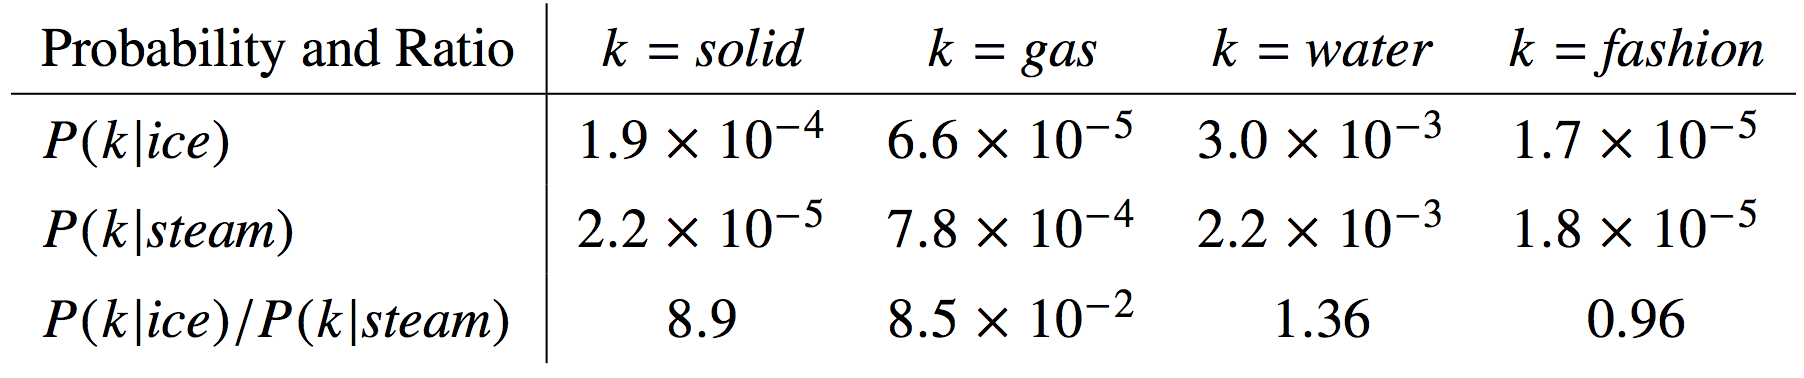
\includegraphics[height=15mm,  width=75mm]{figures/4_glovetable.png}
		\caption[Co-occurrence probabilities for target words]{Co-occurrence probabilities for target words ice and steam with selected context words f}
			\label{glovetable}
\end{figure}

Now considering two words i = ice and j = steam, The relationship of these words ~\autoref{glovetable} can be examined by studying the ratio of their co-occurrence probabilities with various probe words, k. For words k related to ice but not steam, say k = solid, we expect the ratio ${P}_{ik} /{P}_{jk}$ will be large. Similarly, for words k related to steam but not ice, say k = gas, the ratio should be small. For words k like water or fashion, that are either related to both ice and steam, or to neither, the ratio should be close to one. As compared to raw probabilities, the ratio is better able to distinguish relevant words (solid and gas) from irrelevant words (water and fashion) and it is also better able to discriminate between the two relevant words.

As the ratio ${P}_{ik} /{P}_{jk}$ depends on three words i, j and k, the most general model takes the form:
\begin{center}
$F({w}_{i},{w}_{j},{\tilde{w}}_{k}) = \frac{{P}_{ik}}{{P}_{jk}}$
\end{center}

\section{Polyglot}
\section{Paragraph Vectors}
\chapter{Deep Learning: Modern Apporaches}\label{chapter:modernapproach}

\section{RNTN : Recursive Neural Tensor Networks}
\section{MSDA : Marginalized Stacked Denoising Auto Encoders}
\section{CNN : Convoluted Neural Networks}
\section{LSTM : Long and Short Term Memory Networks}
\section{Comparative Evaluation}
	\chapter{Concatenated Word Representations for Sentiment Classifications}\label{chapter:wordrepresentation}

\section{Section}
Citation test~\parencite{latex}.

\subsection{Subsection}
See~\autoref{fig:sample}.

\begin{figure}[htb]
  \centering
  \includegraphics{logos/tum}
  \caption[Example figure]{An example for a figure.}\label{fig:sample}
\end{figure}

\section{Section}

See~\autoref{tab:sample}, \autoref{fig:sample-drawing}, \autoref{fig:sample-plot}, \autoref{fig:sample-listing}.

\begin{table}[htb]
  \caption[Example table]{An example for a simple table.}\label{tab:sample}
  \centering
  \begin{tabular}{l l l l}
    \toprule
      A & B & C & D \\
    \midrule
      1 & 2 & 1 & 2 \\
      2 & 3 & 2 & 3 \\
    \bottomrule
  \end{tabular}
\end{table}

\begin{figure}[htb]
  \centering
  % This should probably go into a file in figures/
  \begin{tikzpicture}[node distance=3cm]
    \node (R0) {$R_1$};
    \node (R1) [right of=R0] {$R_2$};
    \node (R2) [below of=R1] {$R_4$};
    \node (R3) [below of=R0] {$R_3$};
    \node (R4) [right of=R1] {$R_5$};

    \path[every node]
      (R0) edge (R1)
      (R0) edge (R3)
      (R3) edge (R2)
      (R2) edge (R1)
      (R1) edge (R4);
  \end{tikzpicture}
  \caption[Example drawing]{An example for a simple drawing.}\label{fig:sample-drawing}
\end{figure}

\begin{figure}[htb]
  \centering

  \pgfplotstableset{col sep=&, row sep=\\}
  % This should probably go into a file in data/
  \pgfplotstableread{
    a & b    \\
    1 & 1000 \\
    2 & 1500 \\
    3 & 1600 \\
  }\exampleA
  \pgfplotstableread{
    a & b    \\
    1 & 1200 \\
    2 & 800 \\
    3 & 1400 \\
  }\exampleB
  % This should probably go into a file in figures/
  \begin{tikzpicture}
    \begin{axis}[
        ymin=0,
        legend style={legend pos=south east},
        grid,
        thick,
        ylabel=Y,
        xlabel=X
      ]
      \addplot table[x=a, y=b]{\exampleA};
      \addlegendentry{Example A};
      \addplot table[x=a, y=b]{\exampleB};
      \addlegendentry{Example B};
    \end{axis}
  \end{tikzpicture}
  \caption[Example plot]{An example for a simple plot.}\label{fig:sample-plot}
\end{figure}

\begin{figure}[htb]
  \centering
  \begin{tabular}{c}
  \begin{lstlisting}[language=SQL]
    SELECT * FROM tbl WHERE tbl.str = "str"
  \end{lstlisting}
  \end{tabular}
  \caption[Example listing]{An example for a source code listing.}\label{fig:sample-listing}
\end{figure}

\chapter{Moving from Text to Speech: Emotion Recognition}\label{chapter:emotionrecognition}

\section{Conventional Methods}
 	\subsection{GMM: Gaussian Mixture Models}
 	\subsection{I-Vectors: Total Variability Matrix}
 \section{Deep Neural Networks for Emotion Recognition}
\chapter{Conclusion}\label{chapter:conclusion}

\section{Section}
%Citation test~\parencite{latex}.

\subsection{Subsection}
See~\autoref{fig:sample}.

\begin{figure}[htb]
  \centering
  \includegraphics{logos/tum}
  \caption[Example figure]{An example for a figure.}\label{fig:sample}
\end{figure}

\section{Section}

See~\autoref{tab:sample}, \autoref{fig:sample-drawing}, \autoref{fig:sample-plot}, \autoref{fig:sample-listing}.

\begin{table}[htb]
  \caption[Example table]{An example for a simple table.}\label{tab:sample}
  \centering
  \begin{tabular}{l l l l}
    \toprule
      A & B & C & D \\
    \midrule
      1 & 2 & 1 & 2 \\
      2 & 3 & 2 & 3 \\
    \bottomrule
  \end{tabular}
\end{table}

\begin{figure}[htb]
  \centering
  % This should probably go into a file in figures/
  \begin{tikzpicture}[node distance=3cm]
    \node (R0) {$R_1$};
    \node (R1) [right of=R0] {$R_2$};
    \node (R2) [below of=R1] {$R_4$};
    \node (R3) [below of=R0] {$R_3$};
    \node (R4) [right of=R1] {$R_5$};

    \path[every node]
      (R0) edge (R1)
      (R0) edge (R3)
      (R3) edge (R2)
      (R2) edge (R1)
      (R1) edge (R4);
  \end{tikzpicture}
  \caption[Example drawing]{An example for a simple drawing.}\label{fig:sample-drawing}
\end{figure}

\begin{figure}[htb]
  \centering

  \pgfplotstableset{col sep=&, row sep=\\}
  % This should probably go into a file in data/
  \pgfplotstableread{
    a & b    \\
    1 & 1000 \\
    2 & 1500 \\
    3 & 1600 \\
  }\exampleA
  \pgfplotstableread{
    a & b    \\
    1 & 1200 \\
    2 & 800 \\
    3 & 1400 \\
  }\exampleB
  % This should probably go into a file in figures/
  \begin{tikzpicture}
    \begin{axis}[
        ymin=0,
        legend style={legend pos=south east},
        grid,
        thick,
        ylabel=Y,
        xlabel=X
      ]
      \addplot table[x=a, y=b]{\exampleA};
      \addlegendentry{Example A};
      \addplot table[x=a, y=b]{\exampleB};
      \addlegendentry{Example B};
    \end{axis}
  \end{tikzpicture}
  \caption[Example plot]{An example for a simple plot.}\label{fig:sample-plot}
\end{figure}

\begin{figure}[htb]
  \centering
  \begin{tabular}{c}
  \begin{lstlisting}[language=SQL]
    SELECT * FROM tbl WHERE tbl.str = "str"
  \end{lstlisting}
  \end{tabular}
  \caption[Example listing]{An example for a source code listing.}\label{fig:sample-listing}
\end{figure}

% TODO: add more chapters here

\appendix{}

 % TODO: remove if glossary not needed
\glsaddall{} % add all defined terms to glossary, even if not referenced in text
\printglossaries{}

\microtypesetup{protrusion=false}
\listoffigures{}
\listoftables{}
\microtypesetup{protrusion=true}
\printbibliography[title=References]{}

\end{document}
